% Это основная команда, с которой начинается любой \LaTeX-файл. Она отвечает за тип документа, с которым связаны основные правил оформления текста.
\documentclass{article}

% Здесь идет преамбула документа, тут пишутся команды, которые настраивают LaTeX окружение, подключаете внешние пакеты, определяете свои команды и окружения. В данном случае я это делаю в отдельных файлах, а тут подключаю эти файлы.

% Здесь я подключаю разные стилевые пакеты. Например возможности набирать особые символы или возможность компилировать русский текст. Подробное описание внутри.
\usepackage{packages}

% Здесь я определяю разные окружения, например, теоремы, определения, замечания и так далее. У этих окружений разные стили оформления, кроме того, эти окружения могут быть нумерованными или нет. Все подробно объяснено внутри.
\usepackage{environments}

% Здесь я определяю разные команды, которых нет в LaTeX, но мне нужны, например, команда \tr для обозначения следа матрицы. Или я переопределяю LaTeX команды, которые работают не так, как мне хотелось бы. Типичный пример мнимая и вещественная часть комплексного числа \Im, \Re. В оригинале они выглядят не так, как мы привыкли. Кроме того, \Im еще используется и для обозначения образа линейного отображения. Подробнее описано внутри.
\usepackage{commands}

% Пакет для титульника исследовательского проекта
\usepackage{titlepage}

% Здесь задаем параметры титульной страницы
\setToProgram
\setTitle{3D renderer с нуля}
\setStage{}
\setGroup{192}
%сюда можно воткнуть картинку подписи
\setStudentSgn{}
\setStudent{А.А.Смородинов}
\setStudentDate{03.06.2021}
\setAdvisor{Дмитрий Витальевич Трушин}
\setAdvisorTitle{доцент, к.ф.-м.н.}
\setAdvisorAffiliation{ФКН НИУ ВШЭ}
\setAdvisorDate{}
\setGrade{}
%сюда можно воткнуть картинку подписи
\setAdvisorSgn{}
\setYear{2021}


% С этого момента начинается текст документа
\begin{document}

% Эта команда создает титульную страницу
\makeTitlePage

% Здесь будет автоматически генерироваться содержание документа
\tableofcontents

% Данное окружение оформляет аннотацию: краткое описание текста выделенным абзацем после заголовка
\begin{abstract}
Задача проекта - изучить и реализовать алгоритмы отрисовки трёхмерных объектов на экране, в итоге должна быть написано с нуля приложение, в котором пользователь может взаимодействовать с трёхмерной сценой, задавать различные режимы отрисовки для объектов сцены, менять параметры освещения, источников света, камеры и экрана в реальном времени. При этом программа должна иметь минимальное количество зависимостей от сторонних библиотек.
\end{abstract}

\pagebreak
\section{Введение}
Основная задача проекта - это изучение и реализация основных алгоритмов, использующихся в компьютерной графике, на которых основаны большинство программ 3d моделирования, 3d игр, 3d/VR симуляторов и других приложений, имеющих какое-либо отношение к трёхмерной графике. Помимо этого необходимо изложить теоретические основы этих алгоритмов, описать детали их реализации, написать сопроводительную документацию к коду и протестировать его.

\subsection{Алгоритмы, которые необходимо изучить и реализовать}
\begin{enumerate}
	\item Построение матрицы перехода из глобальной системы координат в пространство камеры
	\item Построение матриц проекции на экран (перспективная и ортогональная проекции)
	\item Удаление фрагментов треугольников, лежащих вне пирамиды зрения (view frustrum)
	\item Проверка точек на глубину с помощью z-буффера (при отрисовке объектов должны отрисовываться только ближайшие объекты к камере, но не те, которые находятся за ними)
	\item Отрисовка отрезков на экране (алгоритм Брезенхэма)
	\item Отрисовка треугольников на экране
	\item Перспективно правильная интерполяция параметров объектов при перспективной проекции
\end{enumerate}
\subsection{Что сделано в проекте}
На данный момент все перечисленные выше алгоритмы реализованы и также написано приложение, в котором пользователь может управлять камерой, перемещаясь по 3d сцене. \\
В сцену можно добавлять 3d модели, загружая их с диска в формате wavefront obj ~\cite{obj}. \\
Поддерживаются только модели с треугольными гранями, в .obj файле может храниться только один объект. \\
Загрузка материалов из .mtl файла не реализована, но для модели можно вручную выбрать карту нормалей и диффузную карту (normal map и diffuse map).

\subsection {Репозиторий}
Репозиторий проекта: ~\cite{3dRenderer}

% Note also that very recently several constructions of~\cite{Elkik73} were clarified and simplified by Gabber and Ramero in~\cite[Chapter~5]{GabRam}.

\pagebreak

\section{Описание функциональных и нефункциональных требований к программному проекту}

% Этот пункт нужен только для программных проектов. В нем вы описываете, что у вас вообще должна быть за программа. На каком языке вы ее пишите. Что она должна делать. Подробное описание. Например, у вас пишется библиотека для работы с многочленами. Она должна предоставлять такие-то классы, пример использования. Она предоставляет такие-то методы, пример использования. Такая-то сложность методов. Например, еще можно написать, что вы тестируете библиотеку с помощью консольного приложения, данные считываются так-то, тестируются такие-то вещи, такие-то вещи выводятся. И так далее и тому подобное.

\subsection{Функциональные требования}
\begin{enumerate}
\item Результат проекта - интерактивное приложение, доступное на windows/linux, в котором пользователь может
\begin{itemize}
	\item просматривать различные 3d сцены, управляя камерой с клавиатуры
	\item настраивать параметры сцены
	\item открывать и добавлять в сцену 3d объекты, сохранённые в различных форматах (на данный момент реализована загрузка простейших 3D моделей в формате wavefront obj ~\cite{obj})
\end{itemize}
	\item В коде должны быть реализованы следующие классы:
	\begin{itemize}
		\item Object
		\item World
		\item Screen
		\item Camera
		\item Renderer
	\end{itemize}
\end{enumerate}

\subsection{Нефункциональные требования}
\begin{enumerate}
	\item Требования к надёжности. При отсутствии файлов данных на диске, или их некорректном формате (файлы изображений, 3d моделей, использующихся приложением) программа сообщает пользователю об ошибке и завершает работу.
	\item Требования к техническим средствам пользователя. 
		\begin{itemize}
			\item Операционная система - windows 10 (в будущем возможно будет добавлена поддержка linux).
			\item Место на диске - сама программа занимает несколько мегабайт. Также необходимо место для файлов данных (3d модели, текстуры, шрифты) - зависит от отрисовываемой сцены, но для небольших сцен также достаточно несколько мегабайт.
			\item Количество ядер процессора - хотя бы одно.
			\item Объём оперативной памяти - хотя бы 1 гигабайт (сама программа требует несколько сотен мегабайт).
		\end{itemize}
	\item Требования к коду
	\begin{itemize}
	\item Каждый класс и функция в программе должны быть документированы и протестированы
	\item Между классами должно быть минимальное количество зависимостей, каждый класс должен выполнять свою конкретную функцию
	\item Разрешается использовать библиотеку для кроссплатформенной отрисовки буфера кадра на экране (например SFML - ~\cite{sfml}), библиотеку для работы с матрицами (glm -  ~\cite{glm}) и библиотеку для загрузки изображений в различных форматах (stb\textunderscore image - ~\cite{stb})
	\end{itemize}
	\item Язык программирования - C++
	\item Используемые библиотеки (статическая линковка)
		\begin{itemize}
			\item glm 0.9.9 ~\cite{glm}
			\item sfml 2.5.1 ~\cite{sfml}
			\item stb\textunderscore image 2.26 ~\cite{stb}
		\end{itemize}
	\item Система поддержки версий - git
	\item Линтер/форматтер - clang format, настройки основаны на google codestyle
	\item Для сборки проекта используется IDE Microsoft Visual Studio 2019
\end{enumerate}

\pagebreak

\section{Краткое описание работы алгоритмов, применяющихся в проекте}
%Здесь идет планомерное изложение информации от начала до конца. Тут не нужна никакая философия или объяснения, все это было во введении. Тут сухой математический текст с определениями, формулировками и где надо доказательствами. Содержательную часть можно бить на части, чтобы структурировать изложение.


%\subsection{Содержательная часть 1}

%\subsection{Содержательная часть 2}

Далее будет представлено сжатое описание работы 3d рендерера. Более подробную информацию можно найти в книгах ~\cite{LRN} и ~\cite{Math3d}, если читатель захочет ознакомится более глубоко с тематикой проекта.

\paragraph{Формат и структура объектов}
$\text{}$\\
В самом простом случае можно считать, что каждый объект сцены - это трёхмерное тело, которое мы аппроксимируем многогранником, или их объединением. 

Каждый многогранник, который мы отрисовываем, будем просто считать набором многоугольников, т.е. сделаем переход от объёмного объекта к его двумерной оболочке. 
Более того, все многоугольники можно триангулировать, поэтому в нашей модели можно считать, что объекты сцены - это просто наборы треугольников. 

На практике обычно разделяют понятия объекта и его 3d модели. Объект - это не только некоторая модель, но также её позиция и ориентация в пространстве, а также другие дополнительные атрибуты. Такой подход позволяет хранить только один экземпляр модели, даже если в сцене участвует несколько объектов, использующих её. В этом случае говорят, что координаты вершин треугольников 3d модели лежат в локальной системе координат. 

В проекте объекты именно так и реализованы: каждый объект содержит в себе 3D модель (набор треугольников с текстурными координатами), свою позицию (трёхмерный вектор), ориентацию (кватернион), коэффициенты масштабирования по осям x,y,z.

\paragraph{Преобразование систем координат}
$\text{}$\\
Для того, чтобы получить координаты треугольников в глобальной системе координат, нужно применить к координатам в локальной системе координат несколько преобразований.

Применив линейный оператор к вектору в $\R^3$ (то есть домножив его на матрицу $3\times 3$) мы можем выполнить гомотетию (растяжение/сжатие) вектора относительно нуля, а также повернуть его в пространстве произвольным образом относительно нуля, или отразить его относительно плоскости, проходящей через ноль. На самом деле, с помощью применения линейного оператора мы можем выполнить произвольное линейное преобразование, а не только перечисленные ранее и их комбинации. Но тем не менее, мы можем заметить, что такое преобразование, как, например, поворот относительно произвольного ненулевого вектора $v_0$ не является линейным (в векторном пространстве, не в аффинном). Для того, чтобы выполнить такое преобразование, можно сначала вычесть из вектора $v_0$, затем повернуть его относительно нуля и в конце добавить к результату $v_0$, в итоге мы получим оператор $B(v) = A(v-v_0)+v_0=Av+(E-A)v_0=Av+v_1$.

Данный формат преобразований не очень удобен тем, что в случае линейных операторов их композиция считается как просто произведение матриц, а здесь композиция операторов считается менее тривиально: $B_1(v)=A_1v+t_1$, $B_2(v)=A_2v + t_2$ $\Rightarrow$ $C(v) = B_2(B_1(v))=(A_2A_1)v + A_2t_1 + t_2$.

Обычно для преобразования координат используют более элегантный способ:
\begin{enumerate} 
	\item По трёхмерному вектору $v=\begin{pmatrix}
x \\ y \\ z
\end{pmatrix}$ строится вектор $v'=\begin{pmatrix}
x \\ y \\ z \\ 1
\end{pmatrix}$
	\item По оператору $B(v)=Av+t$ строится матрица $B' = \begin{bmatrix}
	A & t \\
	0 & 1
	\end{bmatrix}$
	\item Тогда $B'v' = \begin{pmatrix}
	Av + t \\
	1
	\end{pmatrix} = \begin{pmatrix}
	B(v) \\
	1
	\end{pmatrix}$
\end{enumerate}

Таким образом, мы свели произвольное перобразования $\R^3$ вида $B(x)=Ax+t$ к линейному оператору на $\R^4$, где координата $w$ вектора (четвёртая координата) равна $1$.

\pagebreak

\paragraph{Переход в пространство камеры}
$\text{}$\\
После того, как мы получили координаты вершин треугольников в глобальной системе координат, их необходимо перевести в систему координат камеры, то есть нужно так преобразовать $R^3$, чтобы фокус камеры камеры перешёл в начало координат, а вектор направления камеры перешёл в вектор $(0, 0, -1)^T$ (можно было выбрать и другой вектор, это просто вопрос соглашения, главное чтобы он был единичной длины и перпендикулярен вектору, который мы считаем направленным вверх). 

\begin{SCfigure}[0.5][h]
	\caption{Пространство камеры, картинка взята из ~\cite{Math3d}. \\ Прямоугольник - это экран, на который будет проецироваться картинка, точка $O$ - фокус камеры.}
	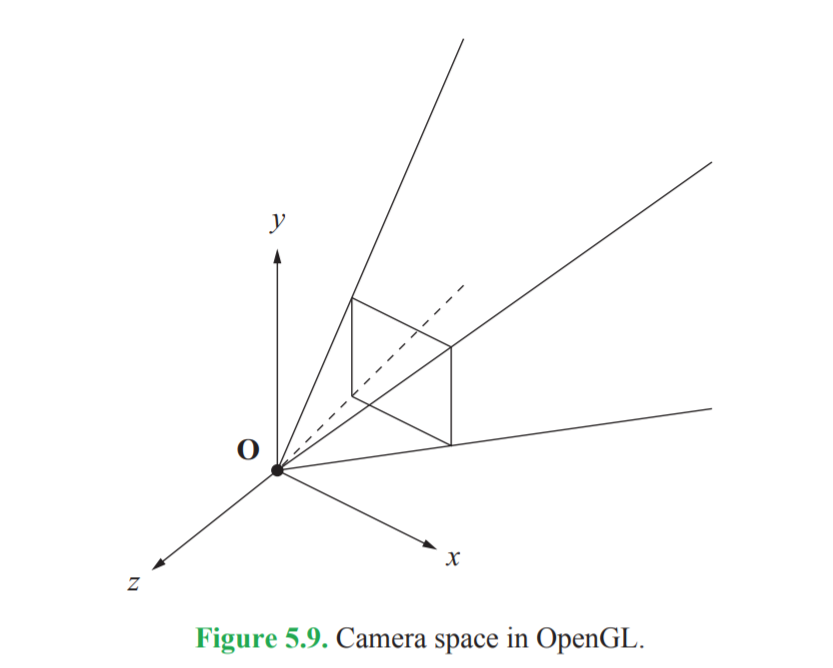
\includegraphics[width=0.5\textwidth]{img1.png}
\end{SCfigure}

Здесь следует отдельно написать, что такое ''вектор направления камеры''. На самом деле, это  просто вектор, который лежит на луче, соединяющем центр камеры с точкой (любой), которая будет проецироваться в центр экрана. Если мы нормализуем данный вектор, то, т.к. мы не хотим растяжения пространства в процессе перехода между системами координат, результирующий вектор также должен будет иметь длину 1.

Это преобразование является композицией поворота и параллельного переноса, поэтому его можно выразить в виде матрицы $4\times 4$ как в прошлом абзаце. Коэффициенты этой матрицы можно посчитать явно, в библиотеке $glm$ ~\cite{glm} эту матрицу можно получить с помощью функции $glm::lookAt(eye, center, up)$, где $eye$ - фокус камеры, $center$ - точка, в которую направлена камера ($center = eye+direction$), $up$ - вектор, который мы считаем направленным вверх, в нашем случае это $(0, 1, 0)^T$.

Теперь, когда у нас есть координаты вершин треугольников в пространстве камеры, осталось лишь спроецировать их на плоскость экрана.

\paragraph{Проецирование на экран}
$\text{}$\\
Всего существует два наиболее распространённых вида проекций - ортографическая и перспективная. В случае ортографической проекции мы просто отбрасываем координату $z$ и получаем в результате вектор $(x, y)^T$ в пространстве экрана. После этого, если мы хотим нормализовать координаты $x, y$, то есть преобразовать их из отрезков $[l, r], [b, t]$ в отрезок $[-1, 1]$, то это можно сделать по формулам $x'=\dfrac{2x-(l+r)}{r-l}$, $y'=\dfrac{2y-(b+t)}{t-b}$

\paragraph{Перспективная проекция}
$\text{}$\\
В случае перспективной проекции, для того, чтобы спроектировать точку \\ $v=(x_0, y_0, z_0)^T$ на двумерный экран, нужно найти пересечение луча $\{tv, t\geq 0\}$ с экраном, задающимся плоскостью $z=-n$ (напоминаю, что в нашей модели направление камеры - это $(0, 0, -1)^T$). 

Также, для того чтобы ограничить возможные значения глубины $z$, вводится так называемая ''дальняя плоскость'', задающаяся уравнением $z=-f$. Все точки, находящиеся за этой плоскостью, то есть имеющие $z<-f$ не будут отрисовываться на экране. Ограничение диапазона возможных значений $z$ позволит нормализовать $z$ и эффективно хранить его с хорошей точностью, при этом расходуя небольшое количество памяти. Зачем вообще нужна координата $z$ станет понятно дальше.

\paragraph{Формулы для вычисления перспективной проекции}
$\text{}$\\
Пусть $(x', y', z')^T \in \{(x, y, z)^T \mid z = -n\} \cap \{tv \mid t\geq 0\}$.

Тогда $x'=\dfrac{-n}{z_0}x_0$, $y'=\dfrac{-n}{z_0}y_0$, $z'=\dfrac{-n}{z_0}z_0=-n$.

Координаты $x', y'$ - это и будут спроецированные координаты точки $v$ на экране. Единственное, что остаётся сделать с ними - это нормализовать, то есть перевести в диапазон $[-1, 1]$. Это нужно просто для удобства дальнейшей работы.

Если мы хотим преобразовать $x$ из диапазона $[a, b]$ в $[-1, 1]$, то это делается с помощью простейшего преобразования: $x'=2\dfrac{x-a}{b-a}-1$

В итоге мы получаем следующие формулы для $x', y'$, если предположить, что экран камеры - это прямоугольник $[l, r]\times[b, t]\times\{-n\} \subseteq \R^3$:

$x'=\dfrac{-2n}{r - l}\big(\dfrac{x_0}{z_0}\big)-\dfrac{r+l}{r-l}$

$y'=\dfrac{-2n}{t - b}\big(\dfrac{y_0}{z_0}\big)-\dfrac{t+b}{t-b}$

Помимо координат $x', y'$ для отрисовки треугольника нам понадобится также координата $z_0$, которая необходима например для того, чтобы определять, какая точка должна отрисовываться на экране, в случае если точек с одинаковыми экранными координатами (полученными после преобразования $x', y'$ в диапазон $[0, screen.width)$, $[0, screen.height)$ и округления их до целого числа) несколько.

\paragraph{Интерполяция координаты z (мотивация для последующих формул)}
$\text{}$\\
Здесь нам придётся забежать немного вперёд, и поговорить об интерполяции. После того, как мы получили координаты $x', y'$ всех вершин треугольника в экранных координатах, мы уже имеем часть необходимых данных, необходимых для отрисовки треугольника на экране. Как было написано выше, нам также понадобится координата $z_0$ для каждой вершины треугольника. 

Треугольник, который мы хотим отрисовать на экране, в результате будет преобразован просто в некоторый набор пикселей. Как уже было написано выше, чтобы понять, какие пиксели реально видимы для камеры, а какие - нет, необходимо знать глубину каждого пикселя треугольника. Но как определить эту глубину? Оказывается, что для того, чтобы найти координату $z$ точки в треугольнике, достаточно знать её барицентрические координаты (об этом и будет следующий абзац) и координаты $z$ вершин треугольника. 
\paragraph{Барицентрические координаты}
$\text{}$\\
\definition Барицентрическими координатами точки $M = (x, y, z)^T$ в треугольнике $ABC$, где $A=(x_0, y_0, z_0)^T, B=(x_1, y_1, z_1)^T, C=(x_2, y_2, z_2)^T$, называется такая тройка чисел $(a, b, c)$, что  $M=aA+bB+cC$, $a,b,c\in[0, 1]$, $a+b+c=1$ 
\begin{lemma}
(без доказательства) \\
$M = (x, y, z)^T \in \triangle ABC$, $A=(x_0, y_0, z_0)^T, B=(x_1, y_1, z_1)^T, C=(x_2, y_2, z_2)^T$, тогда $(a, b, c)$ - бар. координаты точки $M$ $\Rightarrow$  $z=a z_0 + b z_1 + c z_2$. 
\end{lemma}
Т.е. для того, чтобы вычислить координату $z$ точки $M$ нам достаточно знать её барицентрические координаты (по координатам пикселя внутри треугольника барицентрические координаты считаются несложно, здесь эта часть вычислений опущена) и координаты $z_0, z_1, z_2$ вершин треугольника.

Этот подход прекрасно работает в векторных пространствах, но, к сожалению, после проецирования метрика пространства меняется, поэтому $z$ по данной формуле уже нельзя будет считать расстоянием (хотя всё ещё можно использовать для $z$ буфера). В некоторых ситуациях полезно знать расстояние от камеры до объекта, поэтому напрямую это формулу применить нельзя, но есть её альтернатива, которая приводится здесь без доказательства: 

$1/z = a / z_0 + b / z_1 + c / z_2$

Как мы видим, после взятия проекции нужно линейно интерполировать не $z$ а $1/z$

\paragraph{Формулы для вычисления перспективной проекции (продолжение)}
$\text{}$\\
Как мы только что узнали, в процессе растеризации будет необходимо линейно интерполировать $1/z$, поэтому, мы хотим преобразовать $z$ из диапазона $[-f, -n]$ в диапазон $[-1, 1]$($-n \to -1$, $-f \to 1$) (то есть нормализовать) не линейно, а так, чтобы $z'=\dfrac{a}{z}+b$, это позволит интерполировать значения глубины линейно.

Заметим, что $x', y', z'$ зависят от $x, y, 1/z$ следующим образом: $x'=ax/z + b$, $y'=cy/z+d$, $z'=e/z + g$ \\
Пусть $v' = (v'_0, v'_1, v'_2, v'_3)^T=(-x'z, -y'z, -z'z, -z)^T$ \\
Тогда $-x'z = -ax-bz$, $-y'z = -cy-dz$, $-z'z=-e-gz$ $\Rightarrow$ $v' = \begin{bmatrix}
-a & 0 & -b & 0 \\
0 & -c & -d & 0 \\
0 & 0 & -g & -e \\
0 & 0 & -1 & 0
\end{bmatrix} \begin{bmatrix}
x \\ y \\ z \\ 1
\end{bmatrix} = $\\
$=
\begin{bmatrix}
\dfrac{2n}{r-l} & 0 & \dfrac{r+l}{r-l} & 0 \\
0 & \dfrac{2n}{t-b} & \dfrac{t+b}{t-b} & 0 \\
0 & 0 & -\dfrac{f+n}{f-n} & -\dfrac{2nf}{f-n} \\
0 & 0 & -1 & 0
\end{bmatrix} \begin{bmatrix}
x \\ y \\ z \\ 1
\end{bmatrix} =
M v$ \\
Но тогда $x'=v'_0 / v'_3, y' = v'_1 / v'_3, z' = v'_2 / v'_3$.

Резюме: для того, чтобы перевести точку из системы координат камеры в систему нормализованных экранных координат необходимо:
\begin{enumerate}
	\item Дополнить вектор $(x, y, z)^T$ ещё одной координатой - единичкой. В итоге получаем вектор $v=(x, y, z, 1)^T$
	\item Домножить вектор $v$ слева на матрицу $M$: $v'=Mv$ 
	\item Поделить первые три координаты вектора $v'$ на четвёртую координату.
	\item Первые три координаты вектора $v'$ и будут искомыми нормализованными координатами $x', y', z'$.
	\item При этом $v'_3=-z$ нам понадобится позже. ($z$ - координата $z$ точки в пространстве камеры, $v'_3$ - последняя координата вектора $v'$, нумерация с нуля)
\end{enumerate}
После этого шага мы переводим $x', y'$ в экранные координаты.

\paragraph{Растеризация треугольника}
$\text{}$\\
Теперь, когда у нас есть экранные координаты вершин треугольников, мы должны растеризировать треугольники, то есть отрисовать на экране пиксели, лежащие внутри них.
В проекте алгоритм, растеризующий треугольник выглядит так:
\begin{enumerate}
	\item Сначала находим квадрат, в котором лежит треугольник. Левый нижний угол квадрата - это просто $(\min(x_0, x_1, x_2), \min(y_0, y_1, y_2))$. Правый верхний - $(\max(x_0, x_1, x_2), \max(y_0, y_1, y_2))$. \\
	Также введём некоторые обозначения:
	\begin{itemize}
		\item Вершины треугольника имеют координаты $(x_0, y_0, z_0), (x_1, y_1, z_2), (x_2, y_2, z_2)$, где $x, y$ - в экранных координатах, а $z$ - в нормализованных (экранные координаты отличаются от нормализованных тем, что экранные лежат в диапазоне $[0, screen.width - 1]$, или $[0, screen.height - 1]$, а нормализованные - $[-1, 1]$). Ось $x$ направлена вправо, ось $y$ - вверх. 
		\item Барицентрические координаты точки внутри треугольника будем обозначать как $(\alpha, \beta, \gamma)$. 
		\item Координаты $z$ вершин треугольника в пространстве камеры (см. пункт 5 пред. параграфа) будем обозначать как $(w_0, w_1, w_2)$.
	\end{itemize}
	\item После этого для всех пикселей внутри квадрата нужно проверить, лежат ли они внутри треугольника (это можно сделать например используя знаковое расстояние от пикселя до прямых, содержащих стороны треугольника). 
	\item Если пиксель лежит вне треугольника, то мы его пропускаем.
	\item Вычисляем глубину пикселя $z$ с помощью барицентрических координат точки, которой соответствует пиксель, и координат $z_0, z_1, z_2$ (по формуле, находящейся в конце параграфа про барицентр. координаты) 
	\item Сравниваем глубину пикселя с глубиной, записанной в z-буфере (это просто матрица минимальных значений $z$ для каждого пикселя, где минимум берётся по пикселям всех треугольников, отрисованных в текущем кадре до настоящего момента), и если глубина больше чем в z-буфере (точка находится за какой-то другой), то тоже пропускаем данный пиксель. 
	\item Если мы хотим отрисовать не одноцветный треугольник (а например текстурированный), то все необходимые параметры для вычисления цвета пикселя тоже нужно интерполировать. 
	\item Перспективно-правильная интерполяция. (пример)
	\begin{itemize}
		\item На данном этапе алгоритма у нас уже есть достаточно много информации о пикселе треугольника, который мы хотим отрисовать. Нам известны экранные координаты пикселя($x, y$), а также расстояние от точки, которой этот пиксель соответствует, до камеры ($z$). Мы уже ответили на вопрос ''где отрисовывать пиксель?'', но пока ещё не знаем, ''как его отрисовывать?'', а именно, каким цветом.
		\item Если считать, что все треугольники в мире являются одноцветными, то определить цвет пикселя очень легко, это просто константа для каждого треугольника.
		\item Хотя такое предположение упрощает реализацию алгоритма растеризации, оно всё же достаточно сильно ограничивает возможности 3D рендерера. 
		\item Пусть, вместо этого, вместе с каждым треугольником мы будем хранить не только его положение в пространстве, но и так называемые ''текстурные координаты вершин''. Текстурными координатами вершины будет просто являться пара чисел $(u_i, v_i)\in[0, 1]^2$. 
		\item Тогда, зная текстурные координаты вершин треугольника, мы сможем ''наложить'' текстуру (2D изображение) на наш треугольник. Более формально, каждой точке внутри треугольника можно сопоставить точку внутри текстуры (а значит и её цвет), так чтобы вершине $i$ треугольника соответствовала точка на текстуре с координатами $(u_i, v_i)$.
		\item За счёт данной техники, мы сможем отрисовывать не только одноцветные треугольники, но и произвольные цветные изображения, наложенные на них. Это позволит с использованием относительно небольшого числа треугольников создавать достаточно реалистично выглядящие и детализированные 3D модели.
		\item Если немного подумать, то можно придумать достаточно простую формулу, по которой точки треугольника будут переходить в точки текстуры. Так как мы хотим построить взаимооднозначное соответствие между двумя треугольниками, то кажется довольно разумным просто взять за инвариант барицентрические координаты, так как они линейно меняются внутри треугольника, и по ним можно определять, где находится точка относительно вершин треугольника. В итоге формула бы выглядела так: $(u, v) = \alpha(u_0, v_0)+\beta (u_1, v_1)+\gamma(u_2, v_2)$.
		\item К сожалению, такой подход не учитывает искажения перспективной проекции: объекты, находящиеся дальше от камеры на экране становятся меньше, но в треугольнике мы интерполируем текстурные координаты линейно. Например, пусть есть треугольник, одна из вершин которого уходит далеко в бесконечность (ну или просто достаточно далеко). Тогда, по нашей формуле, центр треугольника (пер. медиан) находился бы в центре спроект. треугольника, что показалось бы наблюдателю неестественным, так как этот центр на самом деле расположен очень далеко от нас (а значит должен быть близко к центру экрана, точке схода). К сожалению, мои ограниченные писательские способности плохо позволяют описать этот эффект, с этим гораздо лучше справляется картинка.
		\begin{SCfigure}[0.5][h]
			\caption{Источник: ~\cite{zimg3}.}
			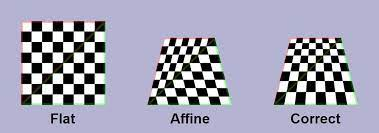
\includegraphics[scale=1]{img2.png}
		\end{SCfigure}
		\item Правильная интерполяция текстурных координат будет вычисляться по формуле \\
		$(u,v) = w\cdot (\alpha (u_0, v_0) / w_0 + \beta (u_1, v_1) / w_1 + \gamma (u_2, v_2) / w_2)$, данный факт приводится без доказательства.
		\item Теперь, зная текстурные координаты точки $(u, v)$, мы можем отрисовать на экране пиксель тем цветом, которому соответствует эта точка на текстуре.
		\item В общем случае, цвет пикселя может определяться не только текстурой, но и различными параметрами освещения (например источниками света), параметрами материала, внешние свойства которого мы хотим передать, и другими вещами. За вычисление цвета отвечает шейдер - алгоритм (программа), который по входным данным (константам и параметрам, интерполирующимся внутри треугольника) определяет цвет пикселя.
	\end{itemize}
	\item Вычисленный цвет пикселя записывается в буфер цветов (матрица цветов пикселей).
	\item Глубина $z$ пикселя записывается в z-буфер.
\end{enumerate}

В результате всех этих операций в итоге мы получим буфер цветов, который и будет выведен на экран.

\section{Детали реализации приложения}

\subsection{Основные классы}
\paragraph{\mintinline{c++}{Application}}
$\text{}$\\
Основной класс приложения - это \mintinline{c++}{Application}. \\
Он хранит в себе классы:
\begin{itemize}
	\item 
	\mintinline{c++}{SFMLRenderer} - 3d рендерер
	\item \mintinline{c++}{UserInterface} - отвечает за вывод на экран отладочной информации
	\item \mintinline{c++}{eng::Scene} - сцена, которая хранит в себе 3d модели, источники света и камеру
	\item \mintinline{c++}{sf::RenderWindow} - SFML окно, на которое отрисовывается 3d сцена и пользовательский интерфейс
	\item \mintinline{c++}{eng::CameraControl} - класс, отвечающий за перемещение камеры пользователем с помощью ввода с клавиатуры
\end{itemize} 

У класса \mintinline{c++}{Application} есть функция \mintinline{c++}{void Application::run()}, которая запускает основной цикл работы, в котором в каждом кадре:
\begin{itemize}
 \item средствами \mintinline{c++}{SFML}~\cite{sfml} обрабатывается ввод пользователя
 \item вызывается метод \mintinline{c++}{size_t SFMLRenderer::render(eng::Scene& scene)} у поля 
 \mintinline{c++}{renderer_}, который отрисовывает сцену на экране и возвращает количество растеризованных треугольников.
 \item собирается и выводится на экран различная статистика о работе программы (например количество кадров в секунду) с помощью класса \mintinline{c++}{UserInterface}
\end{itemize}

В итоге, для запуска приложения достаточно подключить в файле \mintinline{c++}{main.cpp} header \mintinline{c++}{"Application.h"} в функции \mintinline{c++}{void main()} создать класс \mintinline{c++}{Application} и вызвать у него функцию \mintinline{c++}{void Application::run()}. 

Как можно видеть, класс \mintinline{c++}{Application} занимается специфическими для конкретного приложения задачами (обработка ввода пользователя, работа с \mintinline{c++}{SFML}~\cite{sfml}, создание сцены и т.д.), а собственно отрисовку 3D сцены он делегирует классу \mintinline{c++}{SFMLRenderer}

\paragraph{\mintinline{c++}{SFMLRenderer}}
$\text{}$\\
Класс, отвечающий за отрисовку сцены на SFML окне. \\
По сути это просто обёртка над классом \mintinline{c++}{eng::Renderer}, умеющая отрисовывать буфер экрана \mintinline{c++}{eng::Screen} на SFML окне.

\paragraph{\mintinline{c++}{eng::Renderer}}
$\text{}$\\
Класс, ничего не знающий о приложении, которое будет его использовать и конкретном графическом API, используемом для работы с оконной системой. Он умеет отрисовывать объекты сцены (то есть 3d модели, в программе это шаблонный класс \mintinline{c++}{eng::Mesh}) на экране (\mintinline{c++}{eng::Screen}).

\paragraph{\mintinline{c++}{eng::Scene}}
$\text{}$\\
Класс, в котором хранятся объекты сцены (\mintinline{c++}{eng::ObjectsVec}), источники света (\mintinline{c++}{eng::LightsVec}), камера \mintinline{c++}{eng::Camera}

\subsection{Структурная диаграмма классов UML}
\includegraphics[scale=0.15]{diag2.eps}
\subsubsection{Легенда и краткое описание элементов диаграммы}
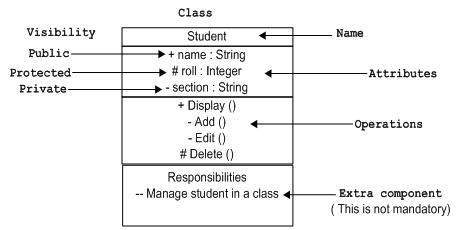
\includegraphics[scale=0.5]{notation_class.jpg}
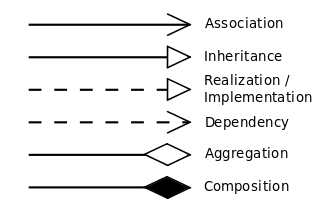
\includegraphics[scale=0.5]{Uml_classes_en.svg.png}\\
Картинки взяты отсюда ~\cite{uml1} и отсюда ~\cite{uml2}. В источнике ~\cite{uml2} достаточно подробно описывается формат UML, если читатель хочет узнать больше про данный формат.
\subsection{Диаграмма потока данных}
\subsubsection{Общая концепция}
Все ресурсы, необходимые для работы программы (текстуры в форматах .png, .jpg, 3d модели в формате .obj, true type шрифт в формате .ttf), загружаются с жёсткого диска в оперативную память. Пользователь взаимодействует с программой с помощью мыши и клавиатуры, программа обрабатывает ввод пользователя и в соответствии с ним обновляет изображение на экране пользователя (на данный момент пользователь может переключать режимы отрисовки объектов, а также управлять камерой).

\subsubsection{Поток данных в каждом кадре}
В каждом кадре программы происходит примерно следующее:
\begin{enumerate}
	\item Класс \mintinline{c++}{Application} обрабатывает события, приходящие от SFML (ввод с клавиатуры, перемещение курсора).
	\item Класс \mintinline{c++}{Application} вызывает у класса \mintinline{c++}{SFMLRenderer} метод \mintinline{c++}{size_t render(eng::Scene& scene)} для отрисовки сцены (сцена как можно видеть передаётся по ссылке).
	\item В результате \mintinline{c++}{SFMLRenderer} вызывает у своего поля \mintinline{c++}{eng::Renderer} метод \mintinline{c++}{size_t renderSceneToScreen(Scene& scene)}, отрисовывающий сцену на экране (сцена снова передаётся по ссылке).
	\item После этого он копирует экран \mintinline{c++}{eng::Screen} попиксельно в текстуру в формате, поддерживаемом SFML, и отрисовывает её на окне SFML.
	\item Класс \mintinline{c++}{Application} вызывает у класса \mintinline{c++}{UserInterface} метод \mintinline{c++}{void updateAndDraw(Seconds deltaTime, size_t trianglesCount)} (никакие данные не копируются).
\end{enumerate}

Как мы видим, данные в программе почти никогда никуда не копируются (кроме копирования экрана в SFML текстуру), а в большинстве случаев просто передаются по ссылкеь.

\section{Тесты на производительность}
На моём компьютере (процессор intel pentium 4415U, 2.3 GHz,  ядра) программа в разрешении 1200x800 в среднем отрисовывает 1 кадр за 200 миллисекунд на сравнительно небольшой сцене с 7400 треугольниками.
% Здесь автоматически генерируется библиография. Первая команда задает стиль оформления библиографии, а вторая указывает на имя файла с расширением bib, в котором находится информация об источниках.

\pagebreak
\bibliographystyle{plainurl}
\bibliography{bibl}



% С этого момента глобальная нумерация идет буквами. Этот раздел я добавил лишь для демонстрации возможностей LaTeX, его можно и нужно удалить и он не нужен для курсового проекта непосредственно.
%\appendix

%Проведем небольшой обзор возможностей \LaTeX. Далее идет обзорный кусок, который надо будет вырезать. Он приведен лишь для демонстрации возможностей \LaTeX.

%\section{Нумеруемый заголовок}
%Текст раздела
%\subsection{Нумеруемый подзаголовок}
%Текст подраздела
%\subsubsection{Нумеруемый подподзаголовок}
%Текст подподраздела

%\section*{Не нумеруемый заголовок}
%Текст раздела
%\subsection*{Не нумеруемый подзаголовок}
%Текст подраздела
%\subsubsection*{Не нумеруемый подподзаголовок}
%Текст подподраздела


%\paragraph{Заголовок абзаца} Текст абзаца

%Формулы в тексте набирают так $x = e^{\pi i}\sqrt{\text{формула}}$. Выключенные не нумерованные формулы набираются либо так:
%\[
%x = e^{\pi i}\sqrt{\text{формула}}
%\]
%Либо так
%$$
%x = e^{\pi i}\sqrt{\text{формула}}
%$$
%Первый способ предпочтительнее при подаче статей в журналы AMS, потому рекомендую привыкать к нему.

%Выключенные нумерованные формулы:
%\begin{equation}\label{Equation1}
% \label{имя-метки} эта команда ставит метку, на которую потом можно сослаться с помощью \ref{имя-метки}. Метки можно ставить на все объекты, у которых есть автоматические счетчики (номера разделов, подразделов, теорем, лемм, формул и т.д.
%x = e^{\pi i}\sqrt{\text{формула}}
%\end{equation}
%Или не нумерованная версия
%\begin{equation*}
%x = e^{\pi i}\sqrt{\text{формула}}
%\end{equation*}

%Уравнение~\ref{Equation1} радостно занумеровано.

%Лесенка для длинных формул
%\begin{multline}
%x = e^{\pi i}\sqrt{\text{очень очень очень длинная формула}}=\\
%\tr A - \sin(\text{еще одна очень очень длинная формула})=\\
%\cos z \Im \varphi(\text{и последняя длинная при длинная формула})
%\end{multline}

%Многострочная формула с центровкой
%\begin{gather}
%x = e^{\pi i}\sqrt{\text{очень очень очень длинная формула}}=\\
%\tr A - \sin(\text{еще одна очень очень длинная формула})=\\
%\cos z \Im \varphi(\text{и последняя длинная при длинная формула})
%\end{gather}

%Многострочная формула с ручным выравниванием. Выравнивание идет по знаку $\&$, который на печать не выводится.
%\begin{align}
%x = &e^{\pi i}\sqrt{\text{очень очень очень длинная формула}}=\\
%&\tr A - \sin(\text{еще одна очень очень длинная формула})=\\
%&\cos z \Im \varphi(\text{и последняя длинная при длинная формула})
%\end{align}

%\begin{theorem}
%Текст теоремы
%\end{theorem}
%\begin{proof}
%В специальном окружении оформляется доказательство.
%\end{proof}

%\begin{theorem}[Имя теоремы]
%Текст теоремы
%\end{theorem}
%\begin{proof}[Доказательство нашей теоремы]
%В специальном окружении оформляется доказательство.
%\end{proof}

%\begin{definition}
%Текст определения
%\end{definition}

%\begin{remark}
%Текст замечания
%\end{remark}

%\paragraph{Перечни:} Нумерованные
%\begin{enumerate}
%\item Первый
%\item Второй
%\begin{enumerate}
%\item Вложенный первый
%\item Вложенный второй
%\end{enumerate}
%\end{enumerate}

%Не нумерованные

%\begin{itemize}
%\item Первый
%\item Второй
%\begin{itemize}
%\item Вложенный первый
%\item Вложенный второй
%\end{itemize}
%\end{itemize}


% Здесь текст документа заканчивается
\end{document}
% Начиная с этого момента весь текст LaTeX игнорирует, можете вставлять любую абракадабру.
